% coordinate 200 in  node (10,200) is too large
% Tried to add edge from (3,4) to (10,200) but node with coordinates (10,200) is not present in the graph
% Tried to add edge from (10,200) to (3,2) but node with coordinates (10,200) is not present in the graph
\documentclass[a4paper,11pt]{article}
\usepackage{mathpazo}
\usepackage{tikz}
\usetikzlibrary{shapes}
\oddsidemargin -0.54cm
\textwidth 17.00cm
\textheight 24cm
\topmargin -1.3cm
\parindent 0pt
\parskip 1ex
\pagestyle{empty}
\begin{document}
\medskip\hrule\medskip

1 1 3 4 10 200 3 2 5 4 are inserted 

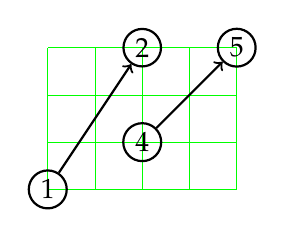
\begin{tikzpicture}[scale=0.600]
\draw [help lines, color=green] (1,1) grid (5,4);

\draw [thick] (1,1) node[draw, rounded rectangle] (0) {1};
\draw [thick] (3,4) node[draw, rounded rectangle] (1) {2};
\draw [thick] (3,2) node[draw, rounded rectangle] (3) {4};
\draw [thick] (5,4) node[draw, rounded rectangle] (4) {5};
\draw [->, thick] (0) to (1);
\draw [->, thick] (3) to (4);

\end{tikzpicture}

\medskip\hrule\medskip
\end{document}
